\chapter{Výsledky} \label{res}
\section{Dopredná neurónová sieť}
Výsledky vyhodnocovania môžeme nájsť v tabuľke \ref{res_fnn}.

\begin{table}[h]
\begin{center}
\begin{tabular}{ c|c|c|c|c|c| } 
 
 Šport (liga) & Tr \% &  Te \% & CG \% & CGP & CGP/M \\ 
 \hline
 Futbal (ENG) & 53,09 & 56,24 & 38,15 & 1,35 & 0,0321 \\ 
 Futbal (GER) & 50,16 & 53,33 & 38,68 & $-0,32$ & $-0,0089$ \\ 
 Futbal (SPA) & 54,24 & 50,76 & 26,86 & $-14,24$ & $-0,2792$ \\ 
 Tenis & 72,8 & 65,2 & 50,82 & $-10,57$ & $-0,0503$ \\ 
 \hline
\end{tabular}
\caption{Priemerné výsledky vyhodnocovania cez 40 iterácií. Skratka Tr \% znamená trénovaciu úspešnosť, Te \% testovaciu úspešnosť. CG značí úspešnosť pri tipovaní zápasov bez favorita, CGP zisk pri uzatváraní stávok na tieto zápasy a CGP/M značí priemerný takýto zisk na zápas bez jasného favorita..}
\label{res_fnn}
\end{center}
\end{table}

\noindent
\begin{figure}[h!]
  \begin{subfigure}[b]{0.48\linewidth}
    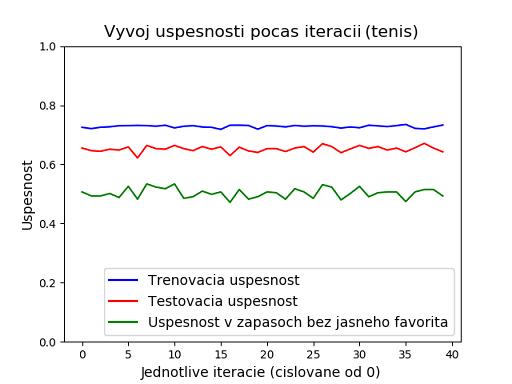
\includegraphics[width=\linewidth]{../img/ffnn_tenis_res.png} 
    \caption{Tenis} 
  \end{subfigure} 
  \begin{subfigure}[b]{0.48\linewidth}
    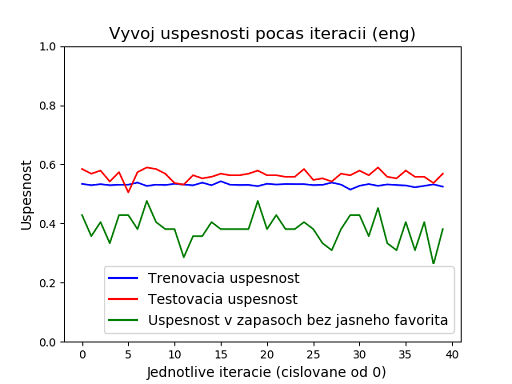
\includegraphics[width=\linewidth]{../img/ffnn_eng_res.png} 
    \caption{Futbal (anglická \textit{Premier league})} 
  \end{subfigure} 
  \begin{subfigure}[b]{0.48\linewidth}
    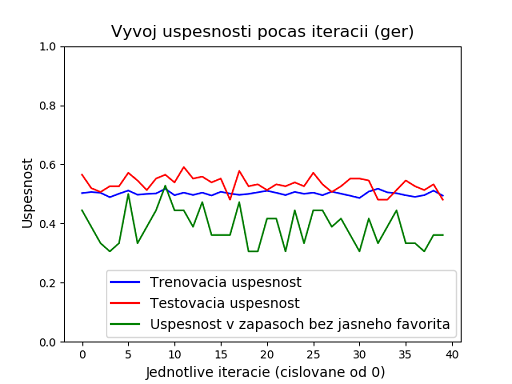
\includegraphics[width=\linewidth]{../img/ffnn_ger_res.png} 
    \caption{Futbal (nemecká \textit{Bundesliga})} 
  \end{subfigure}
  \hfill
  \begin{subfigure}[b]{0.48\linewidth}
    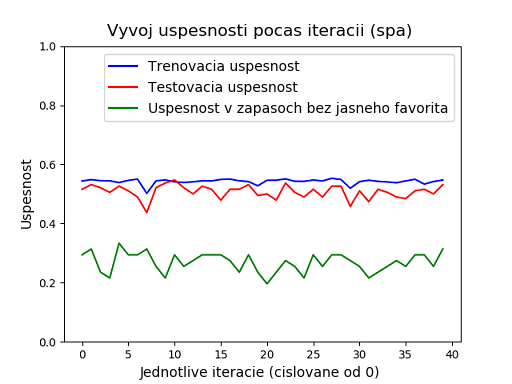
\includegraphics[width=\linewidth]{../img/ffnn_spa_res2.png} 
    \caption{Futbal (španielska \textit{La Liga})} 
  \end{subfigure}
  \caption{Výsledné trénovacie, testovacie úspešnosti a úspešnosti pri predikovaní zápasov bez jasného favorita} 
   \label{fig7} 
\end{figure}

Ak výsledky porovnáme s výsledkami získanými z kapitoly \ref{stavba}, kde sme pre\-di\-ko\-va\-li sezóny pred touto, tak vidíme, že nám sieť vydala iné výsledky.
V prípade tenisu sa to prejavilo mierne horšími hodnotami v sledovaných oblastiach, ale pri zápasoch bez jasného favorita došlo k výraznejšiemu poklesu.

V prípade futbalu pri španielskej lige ako jedinej došlo k poklesu testovacej úspešnosti a obrovský neúspech pre zápasy bez favorita, kde sieť zvolila správny výsledok len pri 26,86\,\% zápasov, čo je dokonca menej ako priemerná úspešnosť pri náhodnom zvolení výsledkov alebo tipovaním len domáceho tímu (obe sú viac ako 33\,\%).
V jednej sezóne sme dokonca dosiahli stratu skoro 25 jednotiek pri tipovaní 51 zápasov a úspešnosti pod 20\,\%, čo značí správne uhádnutých len 10 z 51 zápasov, ktoré v danej sezóne ligy nemali jasného favorita.

Na druhej strane nemecká aj anglická liga sa vyhodnocovali sieti o dosť lepšie ako pri trénovaní, v prípade nemeckej ligy bola testovacia úspešnosť vyššia o 2,5\,\% a v prípade anglickej dokonca o viac ako 5\,\%. Zaujímavosťou je, že úspešnosť v zápasoch bez favorita je na podobnej úrovni ako pri testovaní a celkový zisk sa pohybuje pri oboch ligách okolo 0.

Na obrázkoch \ref{fig7} a \ref{fig8} môžeme vidieť, ako sa vyvíjala trénovacia a testovacia úspešnosť a úspešnosť v zápasoch bez favorita a aký to malo dopad na celkový zisk. Konkrétne na obrázku \ref{fig7} a jeho častiach môžeme vidieť, že jednotlivé úspešnosti boli celkom konzistentné a zatiaľ čo celkové zisky zo zápasov bez favorita sa pohybovali chaotickejšie.


\begin{figure}[h!]
  \begin{subfigure}[b]{0.48\textwidth}
    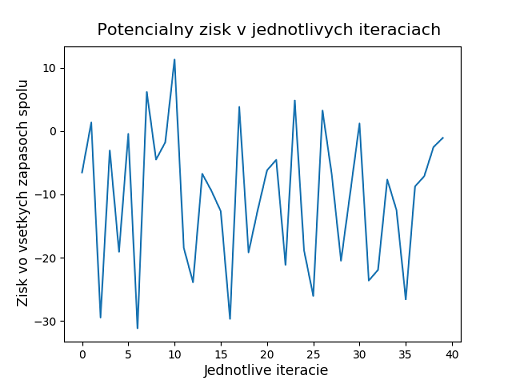
\includegraphics[width=\textwidth]{../img/ffnn_tenis_prof.png} 
    \caption{Tenis} 
  \end{subfigure} 
  \begin{subfigure}[b]{0.48\textwidth}
    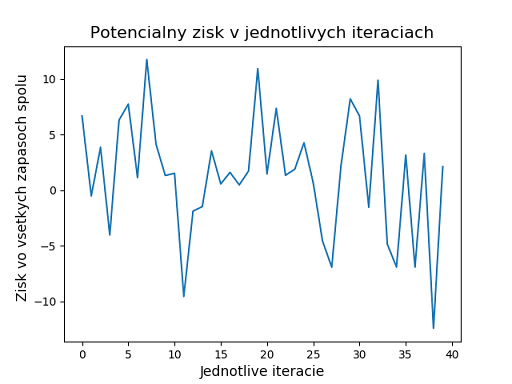
\includegraphics[width=\textwidth]{../img/ffnn_eng_prof.png} 
    \caption{Futbal (anglická \textit{Premier league})} 
  \end{subfigure} 
  \begin{subfigure}[b]{0.48\textwidth}
    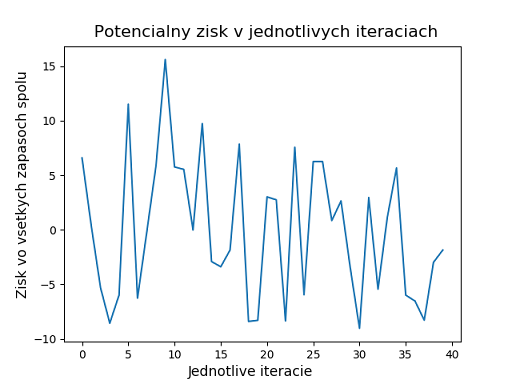
\includegraphics[width=\textwidth]{../img/ffnn_ger_prof.png} 
    \caption{Futbal (nemecká \textit{Bundesliga})} 
  \end{subfigure}
  \hfill
  \begin{subfigure}[b]{0.48\textwidth}
    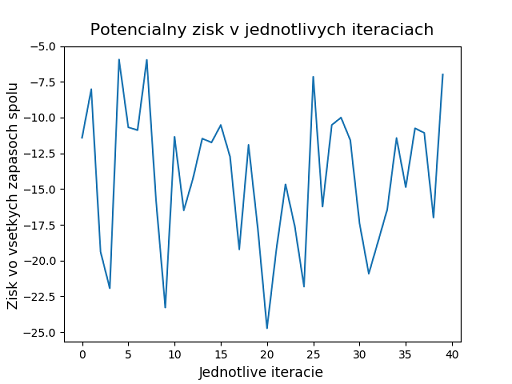
\includegraphics[width=\textwidth]{../img/ffnn_spa_prof.png} 
    \caption{Futbal (španielska \textit{La Liga})} 
  \end{subfigure}
  \caption{Výsledný zisk pri predikovaní zápasov bez jasného favorita (každý šport aj liga mali rôzny počet takýchto zápasov, tento obrázok ukazuje celkový zisk)} 
   \label{fig8} 
\end{figure}

Na obrázku \ref{fig9} môžeme vidieť testovacie úspešnosti pri pre\-dikovaní dvoch sezón, tmavšou farbou sú výsledky z tejto kapitoly, svetlejšou výsledky z kapitoly \ref{stavba}, teda výsledky z testovania a optimalizovania siete.
\begin{figure}[h!]
    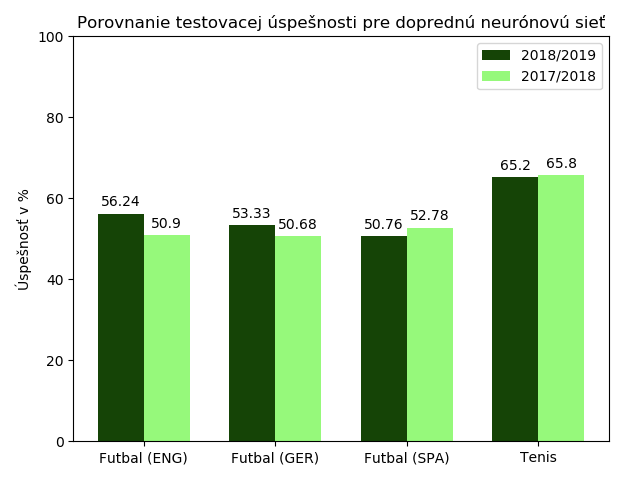
\includegraphics[width=\textwidth]{../img/ffnn_bars.png} 
    \caption{Porovnanie testovacej úspešnosti predikovaní poslednej a predposlednej sezóny. Úspešnosti z predposlednej sezóny (svetlá farba) prebehli pokusom o optimalizáciu a dané dáta aj model použitý pri predikovaní poslednej sezóny (tmavá farba)}
    \label{fig9} 
\end{figure}

\section{Rekurentná neurónová sieť}

Výsledky vyhodnocovania môžeme nájsť v tabuľke \ref{res_rnn}.

\begin{table}[h!]
\begin{center}
\begin{tabular}{ c|c|c|c|c|c| } 
 
 Šport (liga) & Tr \% &  Te \% & CG \% & CGP & CGP/M \\ 
 \hline 
 Futbal (ENG) & 52,44 & 56 & 37 & $-0,12$ & $-0,0029$\\ 
 Futbal (GER) & 49,88 & 50,54 & 38,68 & $-0,1$ & $-0,0028$ \\ 
 Futbal (SPA) & 53,98 & 51,51 & 28,87 & $-12,44$ & $-0,2439$\\
 Tenis & 73,07 & 65,67 & 48,14 & $-22,34$ & $-0,1064$ \\ 
 \hline
\end{tabular}
\caption{Priemerné výsledky vyhodnocovania cez 40 iterácií. Skratka Tr \% znamená trénovaciu úspešnosť, Te \% testovaciu úspešnosť. CG značí úspešnosť pri tipovaní zápasov bez favorita, CGP zisk pri uzatváraní stávok na tieto zápasy a CGP/M značí priemerný takýto zisk na zápas bez jasného favorita.}
\label{res_rnn}
\end{center}
\end{table}

\begin{figure}[h!] 
  \begin{subfigure}[b]{0.48\linewidth}
    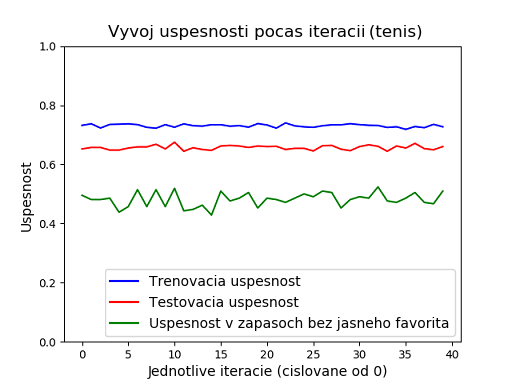
\includegraphics[width=\linewidth]{../img/rnn_tenis_res.png} 
    \caption{Tenis} 
  \end{subfigure} 
  \begin{subfigure}[b]{0.48\linewidth}
    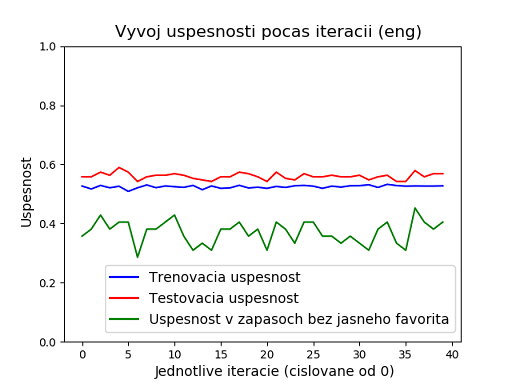
\includegraphics[width=\linewidth]{../img/rnn_eng_res.png} 
    \caption{Futbal (anglická \textit{Premier league})} 
  \end{subfigure} 
  \begin{subfigure}[b]{0.48\linewidth}
    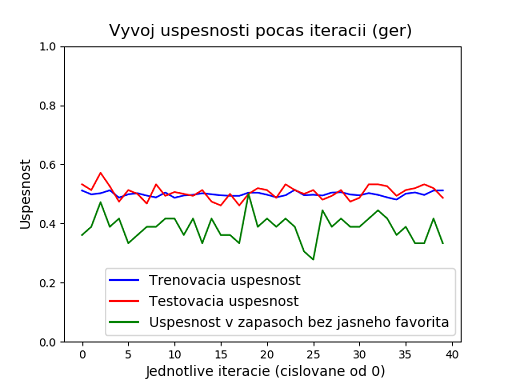
\includegraphics[width=\linewidth]{../img/rnn_ger_res.png} 
    \caption{Futbal (nemecká \textit{Bundesliga})} 
  \end{subfigure}
  \hfill
  \begin{subfigure}[b]{0.48\linewidth}
    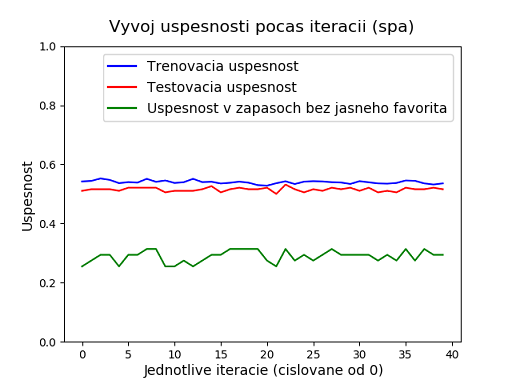
\includegraphics[width=\linewidth]{../img/rnn_spa_res3.png} 
    \caption{Futbal (španielska \textit{La Liga})} 
  \end{subfigure}
  \caption{Výsledné trénovacie, testovacie úspešnosti a úspešnosti pri predikovaní zápasov bez jasného favorita}
   \label{fig10} 
\end{figure}
Ak tieto výsledky porovnáme s výsledkami získanými pri rovnakej architektúre siete, ale pri vynechaní predposlednej sezóny z trénovacích dát a pre\-dikovaní tejto sezóny (sekcia \ref{rnn:train}), tak sa dozvieme, že nie sú až tak odlišné, s výnimkou anglickej futbalovej \textit{Premier league}, kde nastalo zlepšenie z 51,95\,\% na 56\,\%.
Toto zlepšenie ale nastalo na úkor úspešnosti v zápasoch bez jasného favorita, kde pri trénovaní sa dosiahla úspešnosť 39,2\,\% a celkový zisk 2,78 jednotky.

Najvýraznejší pokles oproti trénovaniu nastal v prípade španielskej \textit{La Ligy}, kde pri optimalizovaní siete bola testovacia úspešnosť 53,24\,\%, pri dátach z poslednej ukončenej sezóny dosiahla v priemere sieť úspešnosť 51,51\,\% a pri celkovom zisku pri hypotetickom uzatváraní stávok na zápasy bez favorita dopadla najhoršie z futbalových líg.
Horšie dopadol tenis, ten ale mal väčší počet zápasov bez jasného favorita.
Opäť treba dodať, že úspešnosť španielskej ligy v zápasoch bez favorita bola nižšia ako priemerná náhodná úspešnosť.

V prípade nemeckej \textit{Bundesligy} dopadla pre\-dikcia poslednej sezóny o niečo horšie ako v prípade tej predposlednej, všetky výsledky sú porovnateľné.

Pre tenis dopadla testovacia aj trénovacia úspešnosť mierne horšie, veľký pokles bol v úspešnosti pre\-dikcie zápasov bez favorita, kde prišiel pokles z 52\,\% na 48,14\,\% a to sa prejavilo aj na celkovom zisku v zápasoch bez favorita.

Na obrázkoch \ref{fig10} a \ref{fig11} môžeme vidieť, ako sa vyvíjala trénovacia a testovacia úspešnosť a úspešnosť v zápasoch bez favorita a aký to malo dopad na celkový zisk. Konkrétne na obrázku \ref{fig10} a jeho podobrázkoch môžeme vidieť, že jednotlivé úspešnosti boli celkom konzistentné (s výnimkou úspešnosti v zápasoch bez favorita, kde sa to mierne kolísalo), zatiaľ čo celkové zisky zo zápasov bez favorita (obrázok \ref{fig11}) sa pohybovali chaotickejšie.


\begin{figure}[h!]
  \begin{subfigure}[b]{0.48\textwidth}
    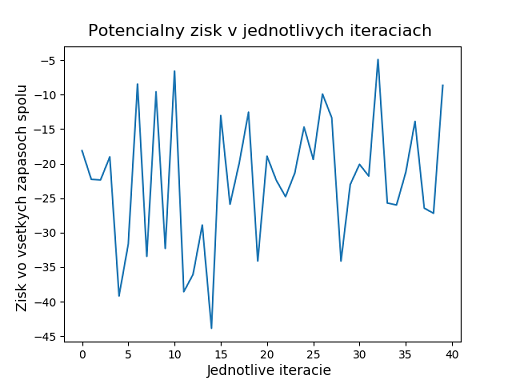
\includegraphics[width=\textwidth]{../img/rnn_tenis_prof.png} 
    \caption{Tenis} 
  \end{subfigure} 
  \begin{subfigure}[b]{0.48\textwidth}
    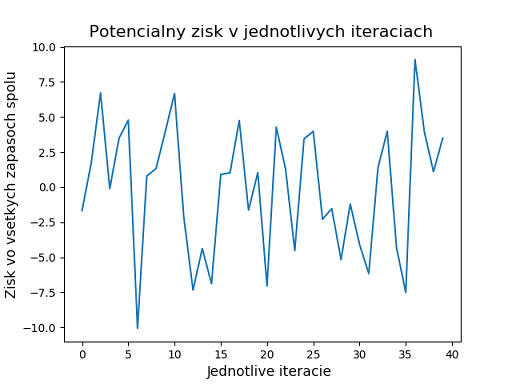
\includegraphics[width=\textwidth]{../img/rnn_eng_prof.png} 
    \caption{Futbal (anglická \textit{Premier league})} 
  \end{subfigure} 
  \begin{subfigure}[b]{0.48\textwidth}
    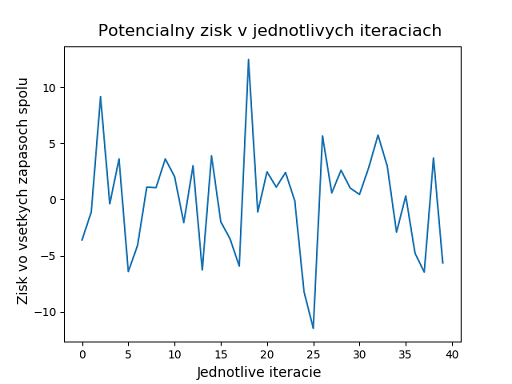
\includegraphics[width=\textwidth]{../img/rnn_ger_prof.png} 
    \caption{Futbal (nemecká \textit{Bundesliga})} 
  \end{subfigure}
  \hfill
  \begin{subfigure}[b]{0.48\textwidth}
    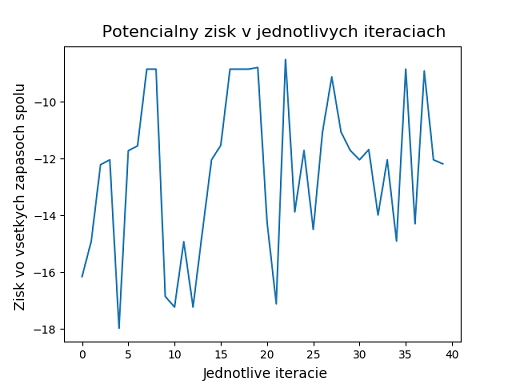
\includegraphics[width=\textwidth]{../img/rnn_spa_prof.png} 
    \caption{Futbal (španielska \textit{La Liga})} 
  \end{subfigure}
  \caption{Výsledný zisk pri predikovaní zápasov bez jasného favorita (každý šport aj liga mali rôzny počet takýchto zápasov, tento obrázok ukazuje celkový zisk)}
   \label{fig11}  
\end{figure}

Na obrázku \ref{fig12} môžeme vidieť testovacie úspešnosti pri pre\-dikovaní dvoch sezón, tmavšou farbou sú výsledky z tejto kapitoly, svetlejšou výsledky z kapitoly \ref{stavba}, teda výsledky z testovania a optimalizovania siete.

\begin{figure}[h!]
    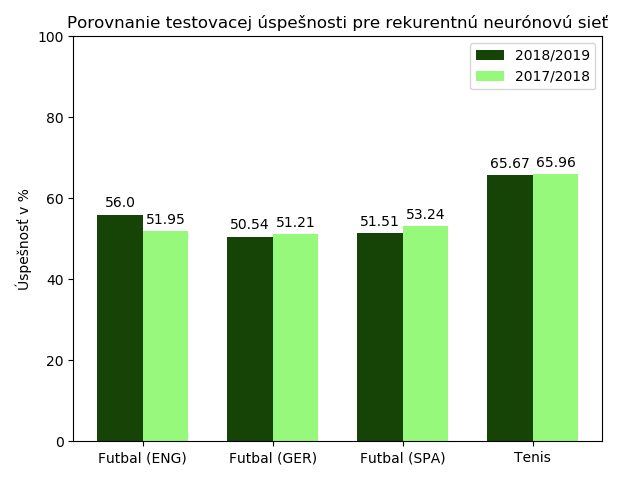
\includegraphics[width=\textwidth]{../img/rnn_bars.png} 
    \caption{Porovnanie testovacej úspešnosti predikovaní poslednej a predposlednej sezóny. Úspešnosti z predposlednej sezóny (svetlá farba) prebehli pokusom o optimalizáciu a dané dáta aj model použitý pri predikovaní poslednej sezóny (tmavá farba)}
    \label{fig12} 
\end{figure}

\section{Porovnanie}
Výsledky dosiahnuté v tejto kapitole boli odlišné, ako výsledky dosiahnuté v kapitole \ref{stavba}.
Videli sme, o koľko sa tieto výsledky líšili.
Môže to značiť mnohé veci, najskôr to ale značí fakt, že každá sezóna má vlastnú predvídateľnosť a aj keď dokážeme sieť naučiť predpovedať jednu sezónu, neznamená to, že rovnaká architektúra bude úspešná aj pri inej sezóne, nie to ešte inej lige alebo športe. V našom prípade sa nám podarilo poraziť stávkové kancelárie len v prípade doprednej neurónovej siete na pre\-dikciu anglickej \textit{Premier League}, aj to len o 1,35 jednotky, čo v preklade znamená, že ak by sme celú sezónu uzatvárali stávky na zápasy bez favorita tak, ako by nám to predpovedala naša sieť a na každý zápas by sme vsadili rovnakú čiastku, tak by sme na konci ostali v zisku, ktorý by sa rovnal 1,35-násobku jedného vkladu.

Na vychýlenie úspešnosti siete vo futbalovej lige zo sezóny na sezónu stačí, ak jeden z dvoch najlepších hráčov sveta prestúpi medzi sezónou do inej ligy a jeho tím nebude bez neho dosahovať rovnaké výsledky \citep{ronaldo}. 
Zdá sa, že obe siete sa v tomto prípade, minimálne zo začiatku sezóny opierali o údaje o dlhodobej sile tímov (príznaky 41 a 42 v Prílohe \ref{in:foot}), čo mohlo viesť k miernemu poklesu úspešnosti tak, ako sme videli.
V anglickej lige sme zaznamenali vzostup aj v trénovacej a aj v testovacej úspešnosti, čo potvrdzuje teóriu o rozličnej predvídateľnosti rozličných sezón.

Zo získaných údajov sme zistili mimo iného aj to, ako sa zmenila predvídateľnosť jednotlivých športových výsledkov z roka na rok (sezóny na sezónu).
Môžeme povedať, že pre\-dikovaná sezóna anglickej \textit{Premier League} bola ľahšie predvídateľná ako tá minulá. Na druhej strane horšie sa obom typom sietí pre\-dikovala španielska \textit{La Liga}. Tieto poznatky môžeme zformulovať do pár hypotéz o rozdiele medzi doprednou a rekurentnou neurónovou sieťou.

Ak je sezóna výrazne horšie predvídateľná ako sezóna, z ktorej sú data, tak oba modely prezentované v tejto práci vykazujú horšie výsledky. Rekurentná neurónová sieť vykazuje mierne lepšie výsledky, LSTM neuróny aj s ich implementáciou krátkodobej pamäte pomáhajú v tomto ohľade sieti.

Naopak, ak je sezóna lepšie predvídateľná ako predchádzajúce, tak obe modely dosahujú vyššej testovacej ako trénovacej úspešnosti. Dopredná neurónová sieť dosahuje o niečo lepšie výsledky, čo môže znamenať, že pamäť rekurentnej neurónovej siete núti túto sieť rozmýšľať konzervatívnejšie.

Celkovo ale sú výsledky veľmi podobné na to, aby sa dali s určitosťou vysloviť nejaké tvrdenia o prezentovaných typoch neurónových sietí.

Na obrázku \ref{fig20} môžeme vidieť rozdiel v úspešnosti medzi najlepšími modelmi doprednej a rekurentnej neurónovej siete podľa kapitoly \ref{stavba} pri pre\-dikcii vyhodnocovanej sezóny (sezóny 2018/2019).

\begin{figure}[t]
    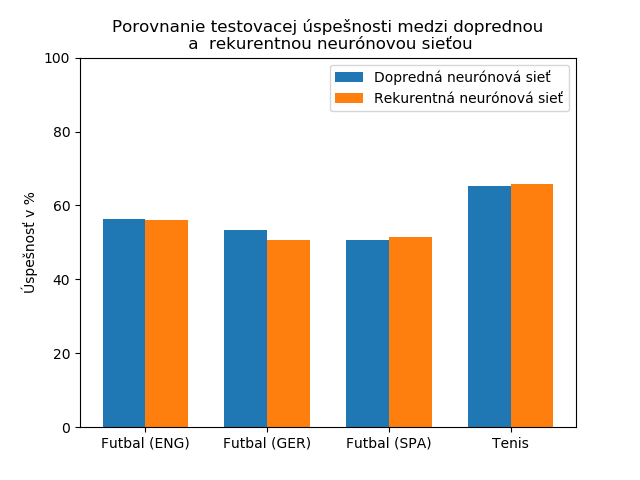
\includegraphics[width=\textwidth]{../img/bars.png} 
    \caption{Porovnanie testovacej úspešnosti modelov doprednej (modrá farba) a rekurentnej (oranžová) neurónovej siete pri predikcii výsledkov jednotlivých líg}
    \label{fig20} 
\end{figure}